\subsubsection{Design Overview of Jefferson lab Electron-Ion Collider}
%VM Design Overview
Jefferson Lab Electron-Ion Collider (JLEIC) is designed as a conventional ring-ring collider.
\cite{Abeyratne:2015pma} The central part of this facility is a set of figure-8 collider rings as shown in Fig. 1. The electron collider ring is made of normal conducting magnets and will store an electron beam of 3 to 10 GeV. The stored electron beam current is up to 3 A and is scaled down when the beam energy exceeds 7 GeV in order to satisfy the operational limit of 10 kW/m synchrotron radiation power. The ion collider ring is made of super-conducting magnets and will store a beam with energy of 8 to 100 GeV for protons or up to 40 GeV per nucleon for heavy ions. The stored ion beam current is up to 0.75 A. The two collider rings are housed in the same underground tunnel. They have nearly identical circumferences of approximately 2.2 km and fit the Jefferson Lab site.

\begin{figure}[!htb]
	\centering
	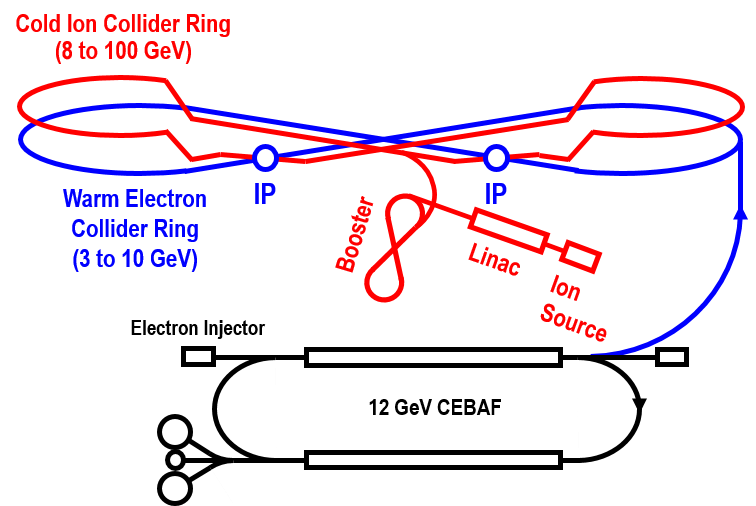
\includegraphics[width=.75\textwidth]{../../img/jleic_schematic.png}
	\caption{Schematic layout of JLEIC}
	\label{fig:jleic1}
\end{figure}

The unique figure-8 shape of the JLEIC collider rings has been chosen to optimally preserve the electron and ion polarizations during acceleration and storage. \cite{Kondratenko:2016eqn}  
Each collider ring is partitioned into two arcs and two long straights. The electron and ion collider rings intersect in the horizontal plane at two symmetric points, one in each of the two long straights as shown in Fig. 1; thus, two detectors can be accommodated. The two long straights also support other utility elements of the collider rings including the beam injection and abort systems, RF accelerating and bunching systems, electron cooler, and beam polarimeters.
The JLEIC design provides a high luminosity exceeding $10^{34}$ cm$^{-2}$ s$^{-1}$ at each interaction point. The high luminosity performance is based on high repetition rate, strong focusing at the collision points, and low beam emittances. The figure-8 design produces over 80\% polarization for both the electron and ion beams and allows for efficient polarization control. Table 1 summarizes some of the high-level design parameters for the machine.

\begin{center}[!htb]
	\begin{tabular}{ l l c c c c } 
		JLEIC Parameters & & \multicolumn{2}{c}{Single-turn ERL Cooler} & \multicolumn{2}{c}{Multi-turn ERL Cooler}\\ 
		& & \multicolumn{2}{c}{PEP-II e-ring} & \multicolumn{2}{c}{New e-ring} \\
		\hline \hline
		& & p & e & p & e\\
		\hline
		Beam energy & GeV & 100 & 5 &100 &5 \\ 
		Collision frequency & MHz& \multicolumn{2}{c}{476} & \multicolumn{2}{c}{476}\\ 
		Particles per bunch & $10^10$ & 0.66 & 3.9& 0.98 & 3.7\\
		Beam current & A & 0.5 & 3 & 0.75 & 2.82\\
		Polarization &  & \textgreater80\% & \textgreater80\% & \textgreater80\% & \textgreater80\%\\
		Bunch length, rms & cm & 1 & 1.2 & 1.2 & 1.2 \\
		Norm. emittance, x/y& $\mu$m & 1/0.5 & 144/72 & 0.5/0.1 & 70/14 \\
		x/y $\beta^*$ & cm &4/2 & 2.6/1.3 & 6/1.2 & 4/0.8\\
		Vert. beam-beam param.& & 0.006 & 0.014 & 0.015 & 0.053\\
		Laslett tune shift & & 0.01 & Small & 0.048 & Small\\
		Detector space, up/down & m & 3.6/7 & 2.4/1.6 & 3.6/7 & 2.4/1.6\\
		Hourglass (HG)reduction & & \multicolumn{2}{c}{0.88} & \multicolumn{2}{c}{0.80}\\
		Lumi./IP, w/ HG, $\mathbf{10^{33}}$ & cm$^{-2}$ s$^{-1}$ & \multicolumn{2}{c}{4.6} & \multicolumn{2}{c}{19.5} \\
		\hline
		%\caption{Parameters and luminosity for a full-acceptance detector.}
		\label{table:parameters}
	\end{tabular}
\end{center}

While thorough background studies must be completed for the specific parameters of the machine, the background issues to be studied in this project are common to any EIC design and the tools and techniques to be developed in this project will be applicable to and allow benchmarking of other EIC designs.

\subsubsection{Full-Acceptance Detector region design}

As illustrated in Figure \ref{fig:detector_concept}, accessing the EIC physics requires reconstruction of a whole event. In particular, one must detect small-angle products including the recoiling target baryon (3D structure of the nucleon), hadrons produced from its breakup (target fragmentation), or all the possible remnants produced when using nuclear targets (including the tagging of spectator protons in polarized deuterium), over a wide range of momenta (and charge-to-mass ratios) with respect to the original ion beam.

From simple kinematics, the reaction products are biased towards small angles around the original ion beam. From machine design and luminosity considerations, it is not desirable to leave a very large detector space free of beam focusing elements to allow the small-angle products to accumulate sufficient transverse separation from the incident beams. The solution is to let the small-angle particles pass through the nearest elements of the machine final-focusing system, which simultaneously perform the function of angle and momentum analyzer for the small angle reaction products. A significant challenge of this approach is that it has to consistently reconcile often contradictory detector and machine optics requirements.

\begin{figure}[!htb]
	\centering
	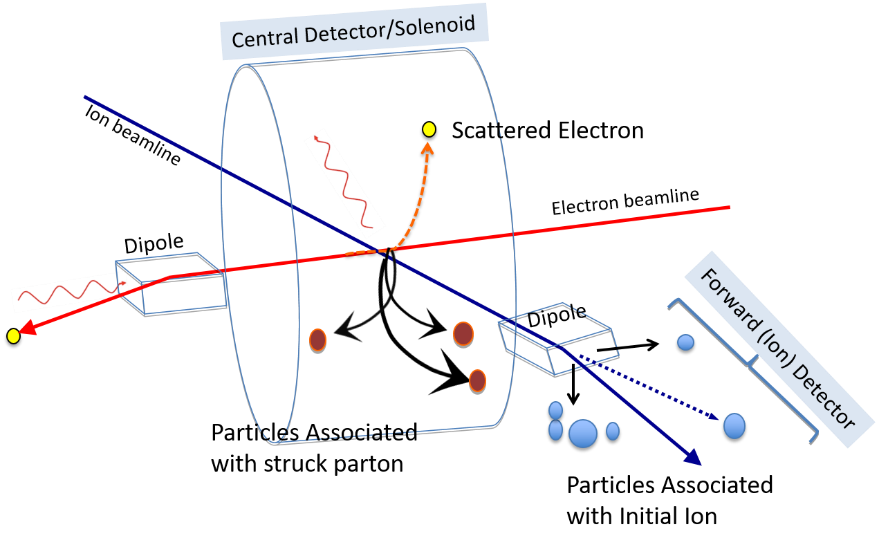
\includegraphics[width=.75\textwidth]{../../img/central_detector.png}
	\caption{Detector concept.}
	\label{fig:detector_concept}
\end{figure}

Figure \ref{fig:detector_schematic} shows a schematic layout of one of the JLEIC interaction regions containing a full-acceptance detector\cite{Abeyratne:2012ah}\cite{Abeyratne:2015pma}\cite{Lin:2013}\cite{Morozov:2012}\cite{Morozov:2014}.  The electron and ion beams cross at a relatively large angle of 50 mrad, which greatly improves the momentum resolution for hadrons detected within a few degrees of the ion beam direction, and provides fast separation of the two beams thus eliminating parasitic bunch collisions and allowing one to move the final focusing elements closer to the interaction point (IP). The electron beam is aligned with the detector axis to avoid generation of synchrotron radiation.


\begin{figure}[!htb]
\centering
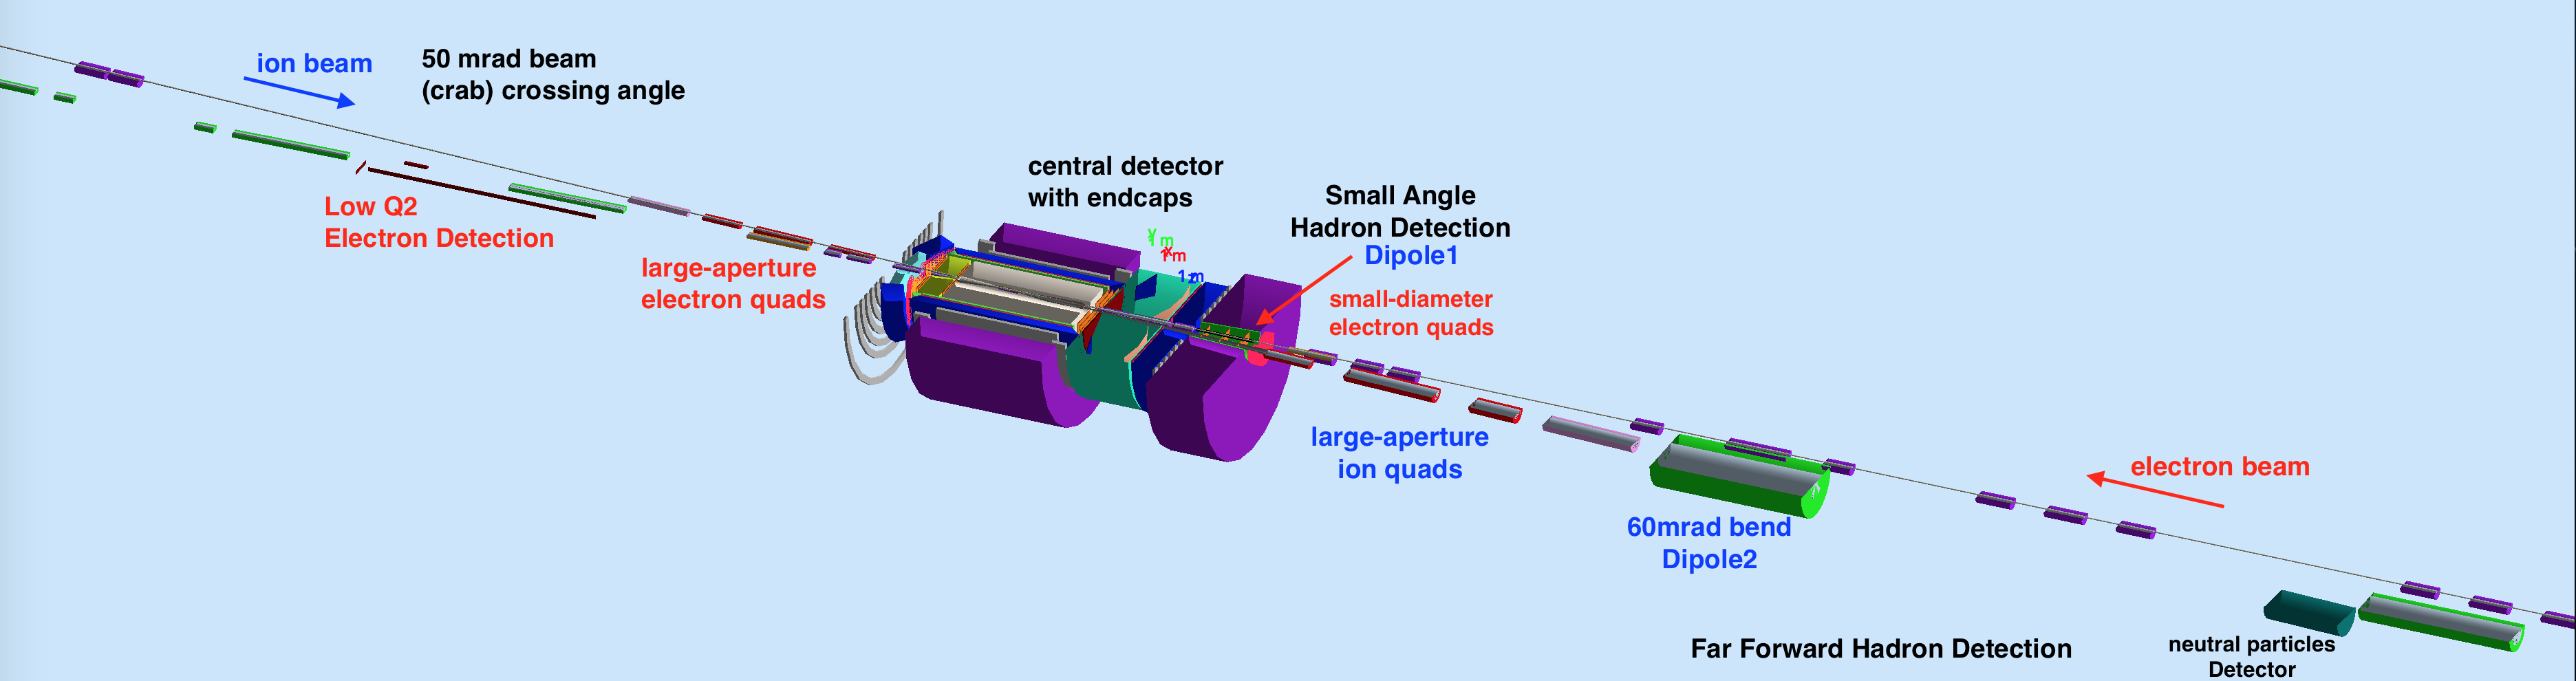
\includegraphics[width=.75\textwidth]{../../img/detector_schematic2.png}
\caption{Schematic layout of the JLEIC full-acceptance detector region.}
\label{fig:detector_schematic}
\end{figure}

The central detector is built around a 4 m long solenoid extending 2.4 m on the outgoing ion side and 1.6 m on the opposite side. The solenoid field is adjustable independently of the beam energies in order to optimize the detection for various processes. The maximum field is expected to be 3 T. The solenoid is surrounded by 2 m long detector end caps. Electrons scattered at small angles ($<0.5^{\circ}$) are detected in a low-Q2 tagger consisting of large-aperture electron Final Focusing Quadrupoles (FFQ) and a spectrometer dipole with a few meters of instrumented space on either side.

In addition to benefiting from the large crossing angle in the solenoid, charged hadrons with scattering angles below $3^{\circ}-5^{\circ}$ with respect to the ion beam will pass through a large-aperture 2 Tm dipole (Dipole 1) located before the ion FFQs. The dipole is 1.5 m long and is followed by 0.5 m of drift space and detectors. Particles at very small angles ($<0.5^{\circ}$)  will pass through the ion FFQs and then, after a few meters of a drift space, through a 56 mrad dipole (Dipole 2) for momentum analysis. Various detector elements are placed in the space between the final focus and Dipole 2 as well as beyond the dipole to provide complete angular and momentum coverage.

The primary full-acceptance detector has a sufficiently large magnet-free space near the interaction point (IP) for detection of particles down to about 0.5 in front of the final focus blocks. In addition, to allow detection of particles scattered between $0^{\circ}-0.5^{\circ}$, the hadrons and electrons need to pass through the large-aperture final focusing quadrupoles and are detected by the further downstream (up to 37 m) detector components \cite{Abeyratne:2012ah} \cite{Abeyratne:2015pma}  \cite{Lin} \cite{Morozov:2012} \cite{Morozov:2014}. 
To maximize the detector’s acceptance to the forwarding scattered hadrons and electrons, both the ion and electron beams are focused downstream of the forward final focus so that small beam sizes at the focal points allow one to place the detectors closer to the beam centers. In combination with ~1 m dispersion at those points, this allows detection of particles with small momentum offset $\Delta p/p$. This optics should be optimized to maximize its angular and momentum acceptance and detector resolution. 

The interaction region optics is optimized to meet the above detection requirements as shown in Figure \ref{fig:ion_magnet_optics} and Figure \ref{fig:ele_magnet_optics} for ions and electrons, respectively. In particular, the detector space is made asymmetric by leaving a large 7 m distance from the IP to the first ion FFQ in the downstream ion direction where the reaction products tend to go, while having the upstream ion FFQs placed closer to the IP at 3.5 m to minimize their chromatic contribution. A weak spectrometer dipole is placed in front of the downstream ion FFQs.

The downstream ion and electron final focusing quads are designed with large apertures for forward detection and are followed by spectrometer dipoles. Additionally, as shown in Figure \ref{fig:magnet_optics}, both the ion and electron beams are focused again towards the ends of the element-free spaces downstream of the respective spectrometer dipoles to allow closer placement of the detectors at those locations, which, in combination with the relatively large dispersion values there, enhances the forward detectors’ momentum resolution. The dispersion generated by the spectrometer dipoles is suppressed on the ion side by a specially designed section, which also controls the beam line geometry, while on the electron side the dispersion suppression is done by a simple dipole chicane whose parameters are chosen to avoid a significant impact on the electron equilibrium emittances. The chicane is designed to accommodate a Compton polarimeter and a luminosity monitor \cite{Morozov:2014}.  Special attention is paid to sizes and positions of the detector region elements to avoid them interfering with each other and with the detector functionality. 

\begin{figure}[!htb]
	\centering
	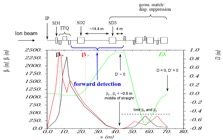
\includegraphics[width=.75\textwidth]{../../img/ion_magnet_optics}
	\caption{Magnetic optics of the ion detector regions.}
	\label{fig:ion_magnet_optics}
\end{figure}

\begin{figure}[!htb]
	\centering	
	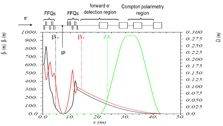
\includegraphics[width=.75\textwidth]{../../img/electron_magnet_optics}	
	\caption{Magnetic optics of the ion and electron detector regions.}
	\label{fig:ele_magnet_optics}
	\end{figure}



The full-acceptance detector region has been integrated into the electron and ion collider ring lattices with necessary optical and geometric matching. As shown in Fig. \ref{fig:jleic1}, the detector is placed far from the electron arc exit to minimize the synchrotron radiation background and close to the ion arc exit to minimize the hadronic background due to the ion beam scattering on the residual gas.

Figure 5 shows an expanded view of the detector region layout. The end section of the ion arc upstream of the IP is shaped to produce a 50 mrad horizontal crossing angle between the ion and electron beams while the ion beam line segment downstream of the IP is designed to produce a 1.5 m transverse separation between the ion and electron beams. The same section is used to suppress the dispersion. The electron detector region has no net bend or shift. This makes the collider ring geometry somewhat independent from the detector region design and simplifies its optimization
 \cite{Lin}.

Due to the strong beam focusing at the IP, the chromatic effect of the FFQs in both the ion and electron collider rings is very significant and requires proper compensation but is manageable. Chromatic compensation is done using properly arranged sextupoles in the rings’ arcs \cite{Nosochkov:2015}.

\begin{figure}[!htb]
	\centering
	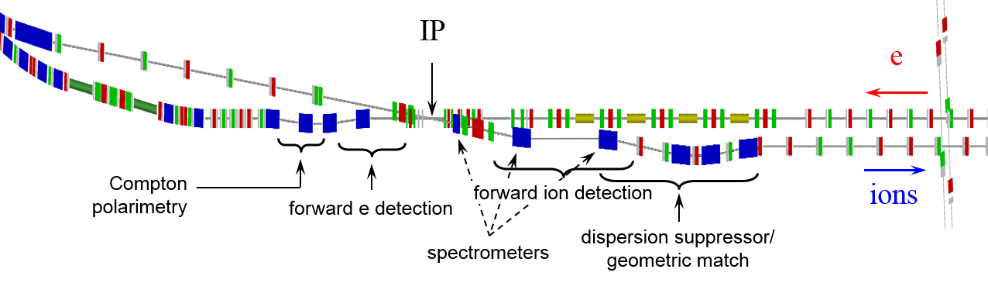
\includegraphics[width=.75\textwidth]{../../img/detector_region_layout}
	\caption{Detector Region Layout}
	\label{fig:detector_region_layout}
\end{figure}